\chapter{Introduction}

\textit{The introduction provides a thorough review of the background, including relevant literature, the motivation, the aims of the thesis and the hypotheses. Literature references for the thesis should be collected in one common bibliography at the end of the thesis.}


\section{Medical Motivation}

\subsection{Anatomy}

\begin{figure}[htbp]
    \begin{minipage}[c][0.9\textheight][t]{.5\textwidth}
        \centering
        \vspace*{\fill}
        \subfloat[The PNS of the upper extremity.]
        {
            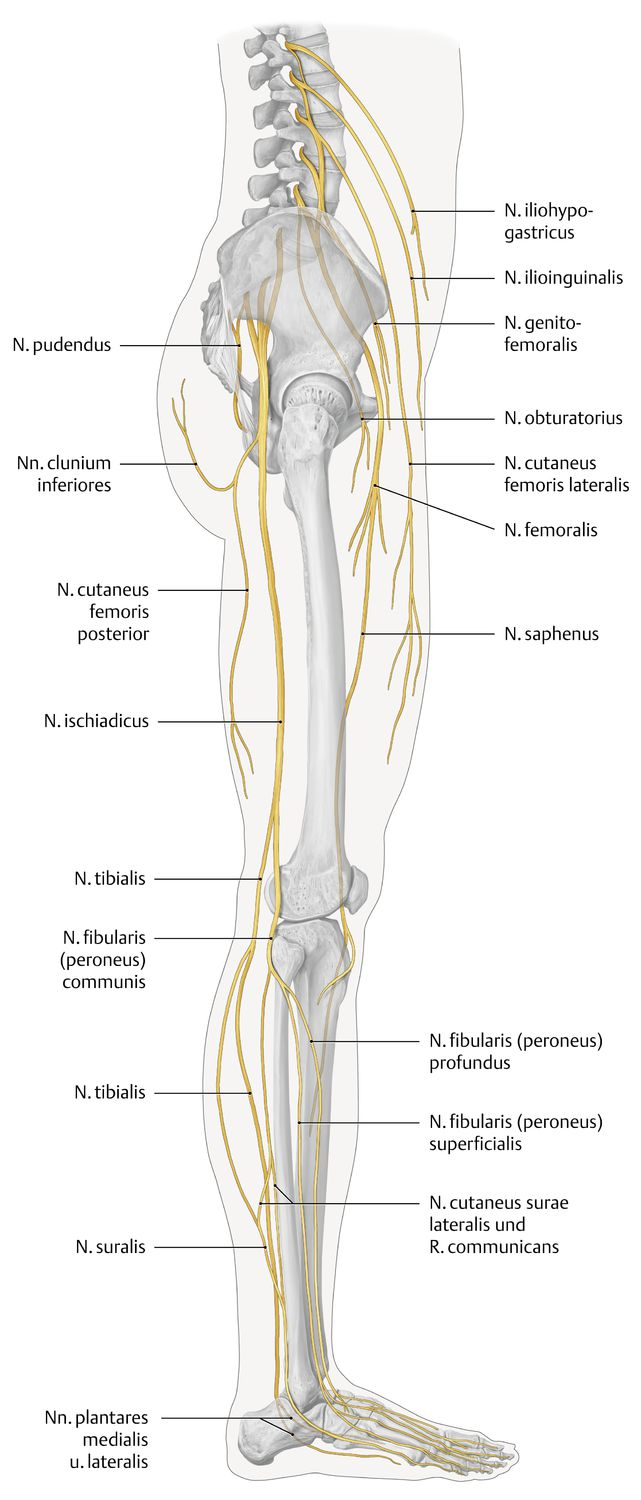
\includegraphics[width=\linewidth]{anat_sagittal}
            \label{fig:subfig:anat_sagittal}
        }
    \end{minipage}
    \begin{minipage}[c][0.9\textheight][t]{.5\textwidth}
        \centering
        \vspace*{\fill}
        \subfloat[Cross-section of the right upper arm (proximal view).]
        {
            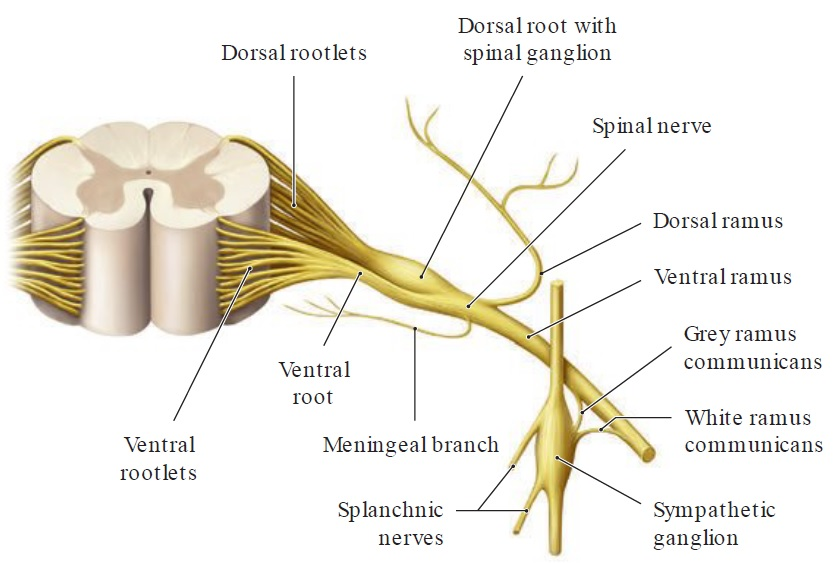
\includegraphics[width=\linewidth]{anat_spinal}
            \label{fig:subfig:anat_spinal}
        }
        \vfill
        \subfloat[Cross-section of the right lower arm (proximal view).]
        {
            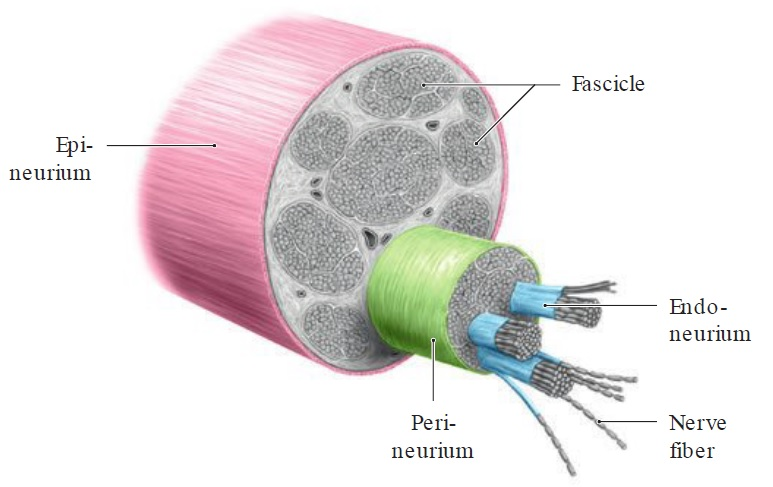
\includegraphics[width=\linewidth]{anat_nerve}
            \label{fig:subfig:anat_nerve}
        }
    \end{minipage}
    \vspace*{-0.3cm}
    \caption[Anatomy of the Peripheral Nervous System of the Lower Extremity]{\textbf{a)} Figure~C p.~537 from~\cite{Schunke2014PrometheusAnatomie}. \textbf{b)} Figure~B p. 384 and \textbf{c)} Figure~D p. 265 from~\cite{Schunke2015THIEMEAnatomy}.}
    \label{fig:anat}
\end{figure}

\begin{figure}[htbp]
	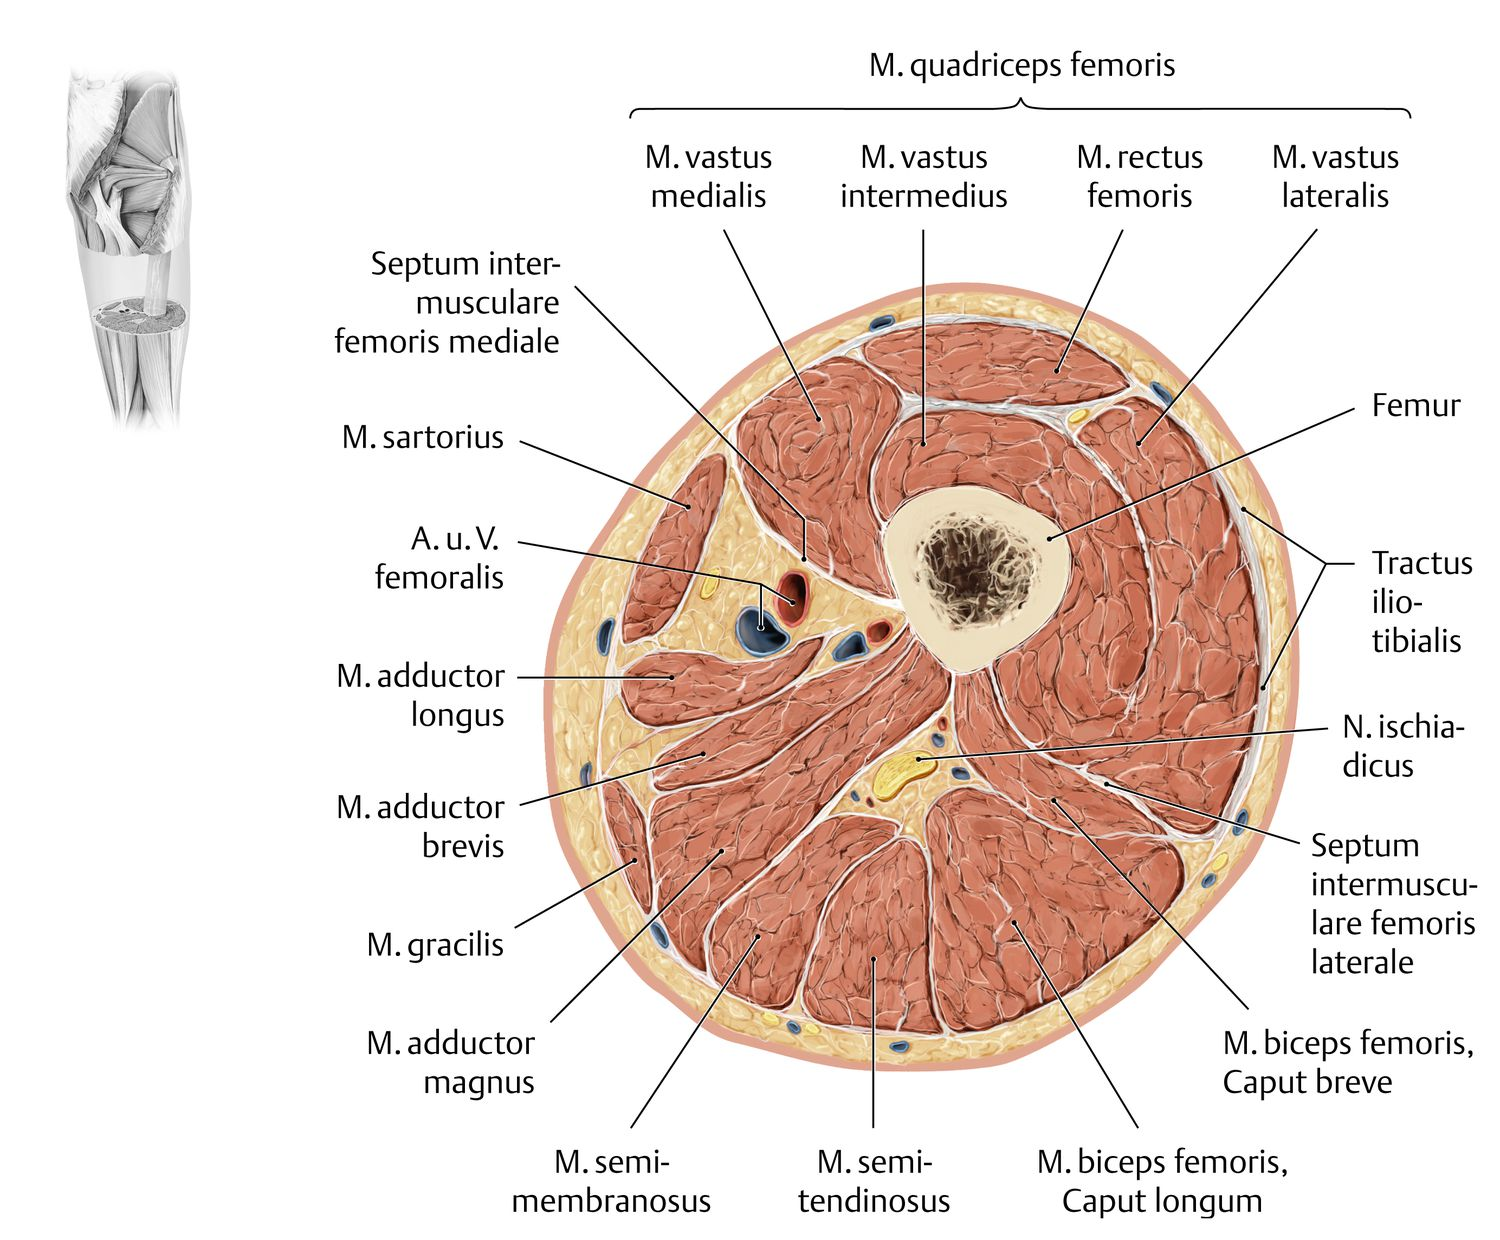
\includegraphics[width=\textwidth]{anat_axial}
    \caption[Cross-section of the Right Upper Leg]{Figure~A p. 528 from~\cite{Schunke2014PrometheusAnatomie}}
    \label{fig:anat_axial}
\end{figure}


\subsection{Peripheral Neuropathies}

\subsection{State-of-the-Art Diagnosis}

\section{Medical Image Segmentation}

\section{Deep Learning}

\subsection{Supervised Learning}
The principle of supervised learning is illustrated on the prediction of house prizes as a function of their living area in Figure~\ref{fig:dl_supervised} and is nicely described in \cite{Ng2012CS229Notes}. In supervised learning, we train an algorithm (or also called model) by showing the algorithm input-output pairs (e.g., living area of houses versus their corresponding prizes). This is referred to as the training phase, and the input-output pairs are called the training set. The main aim of the training phase is to let the algorithm (hopefully) learn a meaningful relationship between the inputs and outputs of our training set. The learned relation, if correct, can then be used to make predictions on previously unseen input data.\\
If the output, we are trying to predict, is continuous, such as in the housing example, the problem is called a regression problem. We could also have the case where we wanted to predict whether the dwelling is an apartment or a house, given the living area. The predicted output would, therefore, be discrete and we would call this a classification problem.\\
Supervised learning gets its name for the reason that the algorithm always learns on input-output pairs (the outputs typically called labels or targets), and the outputs typically are the result of (laborsome) labeling work done by a person. This is the biggest drawback of supervised learning. There, however, exist ways to use unlabeled data in conjunction with labeled data, referred to as semi-supervised learning. Learning on inputs only corresponds to finding patterns and structures in the input space and is referred to as unsupervised learning. Typical examples for unsupervised learning algorithms are \gls{pca} and $k$-means Clustering~\cite{Goodfellow2016DeepLearning}.\\
For the presented example, one could expect a linear relationship between the living area of a house and its prize. If this was indeed true, we could make robust predictions with a simple linear model, only incorporating the living area. However, one could argue that the number of rooms or the location, each with its unknown weight, also influence the dwelling's prize. These influencers are typically called features, and there was and still is a whole science around finding good features to solve learning problems.\\
This is precisely what F. Balsiger did during his master thesis~\cite{Balsiger2016DevelopmentApproaches}: He investigated the different impact features had on the segmentation results of the peripheral nerves done by a trained \gls{rf}~\cite{Breiman2001RandomForests}. The \gls{rf}, also belonging to supervised learning, was trained by engineered features calculated on the \gls{mrn} images, and resulted in a voxel-wise classification into the labels \textit{peripheral nerve} and \textit{background}. \\
The main drawback of any learning algorithm relying on handcrafted features is, however, that the algorithm is inherently constrained by the imagination and ability of the engineer.

\begin{figure}[htbp]
    \centering
	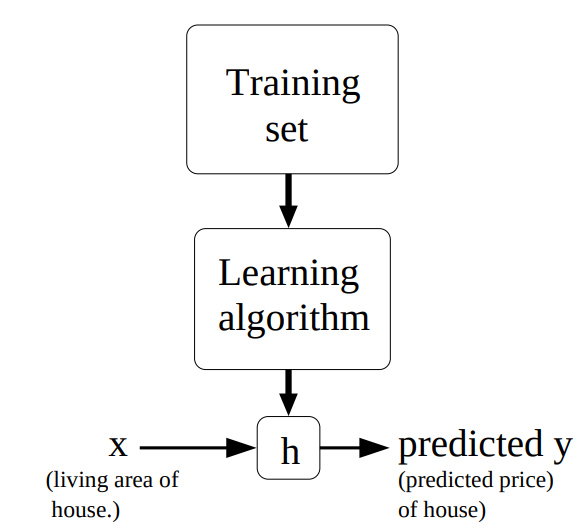
\includegraphics[width=0.5\textwidth]{supervised_learning}
    \caption[Supervised Learning]{The principle of supervised learning illustrated on the example of predicting house prices (y) depending on the living area (x). Suppose we have $m$ area-price pairs, which we name our training set: $\{(x^{(i)}, y^{(i)}); i = 1,...,m\}$. We let $\chi$ and $\upsilon$ denote the space of input and output values, respectively. In this example, $\chi = \upsilon = \mathbb{R}$. In supervised learning we aim to learn a function (also called mapping) $h : \chi \mapsto \upsilon$, which makes reasonable prize prediction (y) for a given new house area (x). We use the training set to learn $h$. Image and example taken from~\cite{Ng2012CS229Notes}.}
    \label{fig:dl_supervised}
\end{figure}

\subsection{Convolutional Neural Networks}



\section{Related Work}
\section{Hypothesis}

\textit{Deep-learning-based segmentation of peripheral nerves from \gls{mrn} images is possible.} \\
\textit{3D-Contextual information allows for better segmentation results.}

\section{Aim \& Structure of the Thesis}

\endinput